\section{Granularity}


As described in Section~\ref{background}, in the standard setting, the inner dimension of each expert network, $\dexp$, is equal to $\dff$, which is the same size as the \ff{} layer of the base model.
\begin{figure*}[t]
  \centering
  \begin{tabular}{ c @{\hspace{30pt}} c }
    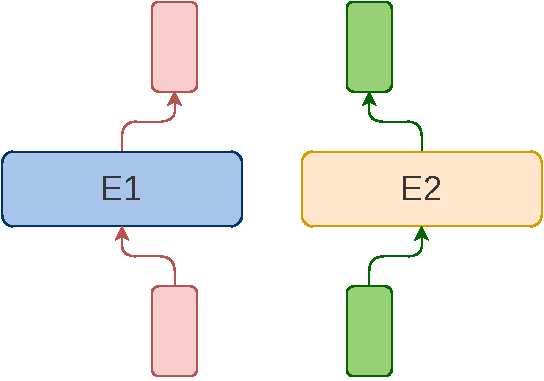
\includegraphics[width=.45\textwidth]{figures/diagram_left_2.pdf} &
      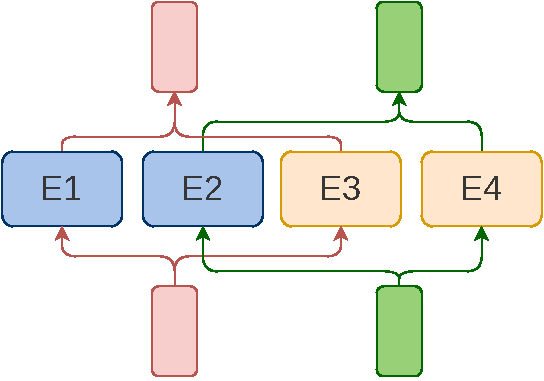
\includegraphics[width=.45\textwidth]{figures/diagram_right_2.pdf} \\
    \small \textbf{(a)} &
      \small \textbf{(b)}
  \end{tabular}

  \medskip

  \caption{\textbf{(a)} Standard MoE layer with $G=1$ \textbf{(b)} Corresponding MoE layer with $G=2$. Each of the original experts is split into two granular ones. The split occurs in the hidden dimension of an expert. Increasing $G$ allows for a more precise mapping between experts and tokens. Since for granularity $G$, the token is routed to $G$ granular experts, the number of parameters activated per token is the same in both cases.}
  \label{diag_gran_better}
\end{figure*}





In this work, we suggest an alternative approach where the hidden dimension of the expert is not necessarily set to mirror that of the standard feed-forward layer. Instead, it can be adjusted to a value that is the most effective. This approach allows the configuration of MoE to be articulated in terms of two key hyperparameters: \textit{granularity} (\(G\)) and \textit{expansion rate} (\(E\)). In the following parts of this work, we will also use the term \textit{active} parameters to refer to the non-embedding parameters used to produce output for a single token, except routing. The number of active parameters is denoted as $\nact$.

Let $\dexpert$ be the hidden dimension of a single expert. Granularity is defined as
\begin{align*}
    G = \frac{\dff}{\dexpert}.
\end{align*}
In other words, granularity denotes the multiplier factor for the change in the size of an expert from the original standard model, defined as $G=1$. 
In this work, we investigate $G > 1$ where experts are smaller than in the standard layer. 

Note that increasing granularity does not affect the number of active parameters. As $G$ increases, the number of experts that process the token grows proportionally to $G$. In other words, for granularity $G$, a token is routed to $G$ fine-grained experts, thereby keeping the number of active parameters constant. See Fig. \ref{diag_gran_better} for visualization.

We then define the \textit{expansion rate}, which describes the increase in the number of parameters from a standard transformer layer to a MoE layer. Given that, $\nmoe$ and $\nff$ denote the total number of parameters in a MoE layer excluding routing and the standard \ff{} layer, respectively. The expansion rate $E$ is then defined as 
\begin{align*}
    E = \frac{\nmoe}{\nff}.
\end{align*}

Expansion rate can also be seen as the total number of parameters in a MoE layer compared to its active parameters. 

The concept of the expansion rate is intricately linked to the number of experts through the idea of granularity. Indeed, the definitions of both granularity and expansion rate extend and refine our understanding of the number of experts, symbolized as $\nexpert$.
\begin{align}
    \nexpert = G \cdot E
\end{align}

For non-granular models, where $G=1$, the expansion rate is equal to the number of experts. 



Intuitively, increasing granularity for a given expansion rate gives the model more flexibility in mapping datapoints to experts, potentially improving performance. We incorporate the notion of granularity into our scaling laws in Section~\ref{sec:scaling_laws}. The discussion about practical tradeoffs in changing this parameter is given in Section~\ref{sec:scaling_app}.

